\section{Setting Preferences} \label{sec:preferences}

Use Morpho preferences to set a Metacat URL, customize the look and feel
of the application, and adjust settings that affect logging and
debugging. Select ``Set preferences...'' under the File menu to open the
Morpho Preferences screen (\autoref{fig:dialog-preferences}).

\begin{figure}
  \centering
    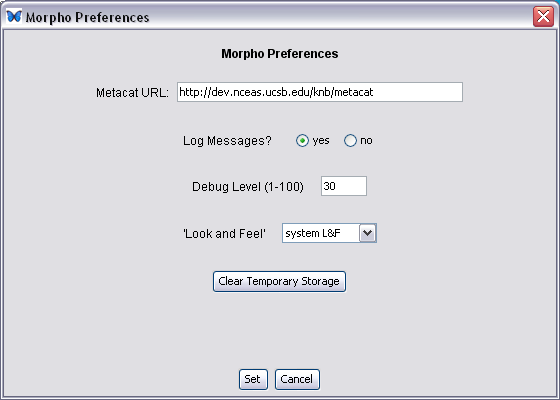
\includegraphics[width=0.7\textwidth]{images/dialog-preferences.png}
  \caption{The Morpho Preferences at the default settings.}
  \label{fig:dialog-preferences}
\end{figure}

\paragraph{Metacat URL} The Metacat URL contains the URL of the network (a Metacat
server) where data are stored. By default, the Metacat URL points to the
KNB Metacat server. Change the default only if you are using a custom
server.

\paragraph{Log Messages} The Log Messages preference, when set to ``yes'' (the
default), specifies that error messages be written to a log file. The
log file is called ``stderr.log'' and can be found in the Morpho startup
directory. If you are experiencing problems with the application,
examining the log file (or sending it to Morpho developers to examine)
may provide clues to the cause. Note that the log file is rewritten
every time Morpho starts up. You must rename the file if you want to
save it.

\paragraph{Debug Level (1-100)} The debug level (set to 30 by default)
configures the debugging level used to log. A level of 1 returns only
the most severe errors. A level of 100 returns every possible error.

\paragraph{Look and Feel} Select an option from the drop-down menu.
``system L\&F'' (the default) instructs Morpho to mimic the look of the
current operating system (e.g., Windows, Mac, etc) ``kunststoff'' is a
customized look-and-feel created for Java applications.

\paragraph{Clear Temporary Storage} The ``Clear Temporary Storage''
option empties the Morpho cache, which contains downloaded data sets.
Under most circumstances, you do not need to use this option. However,
if you have downloaded many large data sets and are running low on hard
drive space, you may wish to use this option. Note that when you clear
the cache, Morpho must re-download each data set the next time you
require it.
